\documentclass[14pt]{extarticle}
\usepackage{amsmath}
\usepackage{amssymb}
\usepackage{graphicx}
%\usepackage{tikz}
%\usetikzlibrary{calc}
%\usetikzlibrary{trees}
\usepackage{graphicx}
\graphicspath{ {../} }
\usepackage[top=0.75in, bottom=0.75in, left=0.75in, right=0.75in]{geometry}
\newcommand*{\Scale}[2][4]{\scalebox{#1}{\ensuremath{#2}}}%
\usepackage[shortlabels]{enumitem}
% \usepackage{showframe}
\title{\vspace{-5ex}HANDOUT Math 208 Week 06}
\date{\vspace{-10ex}}
\usepackage{multicol}
\setlength{\columnsep}{.5cm}

\begin{document}
\maketitle	
\pagenumbering{gobble}	
\section{Counting}
\begin{enumerate}
	\item A class of 50 musicians includes 11 who play the piano, 17 who play the guitar, and 6 who play both the piano and the guitar.
	\begin{enumerate}
		\item How many musicians play neither instrument?
		\vspace{2.2cm}
	\end{enumerate}

	\item A college offers 3 introductory courses in history, 2 in science, 2 in mathematics, 4 in philosophy, and 4 in English.
	\begin{enumerate}
		\item If a freshman takes one course in each area during her first semester, how many course selections are possible?
		\vspace{2.2cm}
		\item If a part-time student can only take one introductory course, how many selections are possible?
		\vspace{2.2cm}
	\end{enumerate}
	\item How many different 5-letter code words can be formed from Q, X, K, V, C, A if no letter is repeated? If letters may be repeated? If adjacent letters must be different?


\cleardoublepage
\section{Permutations and Combinations}
	\begin{multicols}{3}
		$$(7+3)!=$$
		\vspace{0.5cm}
		$$\frac{20!}{18!}=$$
		\vspace{0.5cm}
		$$\frac{10!}{10*9*8!}=$$
		\vspace{0.5cm}
		$$\frac{7!}{8!}=$$
		\vspace{0.5cm}
		$$\frac{9!}{9}=$$
		\vspace{0.5cm}
		$$3!=$$
		\vspace{0.5cm}
	\end{multicols}
	\vspace{0.5cm}
	\begin{multicols}{3}
		$$_{15}C_{10}=$$
		\vspace{0.5cm}
		$$_9P_4=$$
		\vspace{0.5cm}
		$$_{99}C_1=$$
		\vspace{0.5cm}
		$$_{99}P_1=$$
		\vspace{0.5cm}
		$$\frac{_{15}C_{10}}{_{99}C_1}=$$
		\vspace{0.5cm}
	\end{multicols}
	\vspace{2cm}
	\item From a standard 52-card deck, how many 6-card hands consist entirely of clubs?
	\vspace{2cm}
	\\\\
	\item In a horse race, how many different finishes among the first 3 places are possible if 10 horses are running? (Exclude ties.)?
	\vspace{2cm}
\end{enumerate}

\cleardoublepage

\section{Sample Space, Events, and Probability}
\begin{enumerate}
	\item What is the sample space of flipping a coin three times?
	\vspace{2cm}
	\item What is the probability that all three flips will be the same?
	\vspace{2cm}
	\item What is the probability that all three flips will be different?
	\vspace{2cm}
	\item What is the sample space of selecting balls numbered 1-10 from a bin?
	\vspace{2cm}
	\item What is the probability of selecting an prime numbered ball?
	\vspace{2cm}
	\item What is the probability of selecting a ball less than 20?
	\vspace{2cm}
	\item Consider the sample space of a standard deck of cards. What is the probability that I will draw a club?
	\vspace{2cm}
	\item What is the probability I will draw a king or a spade?
	\vspace{2cm}
	\item  Suppose that 6 people check their coats in a checkroom. If all claim checks are lost and the 6 coats are randomly returned, what is the probability that all the people will get their own coats back?
\end{enumerate}


\section{Union, Intersection, etc}
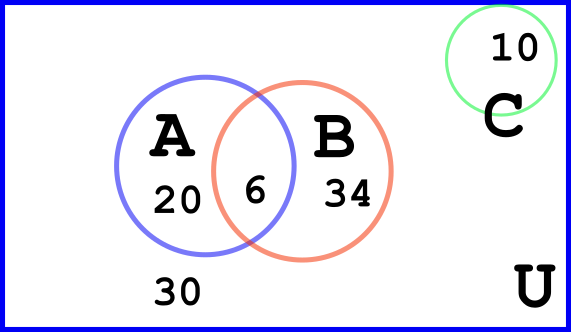
\includegraphics[width=0.5\linewidth]{venn-3}
\begin{multicols}{3}[What are the Probabilities?]
	\begin{enumerate}
		\item $P(A)$
		\vspace{0.5cm}
		\item $P(A\cap B)$
		\vspace{0.5cm}
		\item $P(A\cup B)$
		\vspace{0.5cm}
		\item $P(A')$
		\vspace{0.5cm}
		\item $P(A\cup B')$
		\vspace{0.5cm}
		\item $P(A\cup C)$
	\end{enumerate}
\end{multicols}
\vspace{0.5cm}
\begin{enumerate}\addtocounter{enumi}{6}
	\item When flipping a coin 3 times, what is the probability that the first two flips will be the same or that the last two flips will be the same?
	\vspace{2cm}
	\item When rolling two dice, what is the probability that the result will be odd and less than 7? Prime or greater than 5?
	\vspace{2cm}
	\item What are the odds for rolling 7 or 11?
	\vspace{2cm}
	\item If the odds for E are 3 to 4, what is $P(E)$?
\end{enumerate}


\end{document}
